% (find-LATEX "2021-2-C2-MT2.tex")
% (defun c () (interactive) (find-LATEXsh "lualatex -record 2021-2-C2-MT2.tex" :end))
% (defun C () (interactive) (find-LATEXsh "lualatex 2021-2-C2-MT2.tex" "Success!!!"))
% (defun D () (interactive) (find-pdf-page      "~/LATEX/2021-2-C2-MT2.pdf"))
% (defun d () (interactive) (find-pdftools-page "~/LATEX/2021-2-C2-MT2.pdf"))
% (defun e () (interactive) (find-LATEX "2021-2-C2-MT2.tex"))
% (defun l () (interactive) (find-LATEX "2021-2-C2-MT2.lua"))
% (defun o () (interactive) (find-LATEX "2021-2-C2-MT2.tex"))
% (defun u () (interactive) (find-latex-upload-links "2021-2-C2-MT2"))
% (defun v () (interactive) (find-2a '(e) '(d)))
% (defun d0 () (interactive) (find-ebuffer "2021-2-C2-MT2.pdf"))
% (defun cv () (interactive) (C) (ee-kill-this-buffer) (v) (g))
%          (code-eec-LATEX "2021-2-C2-MT2")
% (find-pdf-page   "~/LATEX/2021-2-C2-MT2.pdf")
% (find-sh0 "cp -v  ~/LATEX/2021-2-C2-MT2.pdf /tmp/")
% (find-sh0 "cp -v  ~/LATEX/2021-2-C2-MT2.pdf /tmp/pen/")
%     (find-xournalpp "/tmp/2021-2-C2-MT2.pdf")
%   file:///home/edrx/LATEX/2021-2-C2-MT2.pdf
%               file:///tmp/2021-2-C2-MT2.pdf
%           file:///tmp/pen/2021-2-C2-MT2.pdf
% http://angg.twu.net/LATEX/2021-2-C2-MT2.pdf
% (find-LATEX "2019.mk")
% (find-CN-aula-links "2021-2-C2-MT2" "2" "c2m212mt2" "c2mt2")

% «.defs»			(to "defs")
% «.title»			(to "title")
% «.regras»			(to "regras")
% «.intro»			(to "intro")
% «.atirei-o-pau-no-gato»	(to "atirei-o-pau-no-gato")
% «.upload-logs»		(to "upload-logs")
% «.lua»			(to "lua")
%
% «.djvuize»			(to "djvuize")



% <videos>
% Video (not yet):
% (find-ssr-links     "c2m212mt2" "2021-2-C2-MT2" "{naoexiste}")
% (code-eevvideo      "c2m212mt2" "2021-2-C2-MT2")
% (code-eevlinksvideo "c2m212mt2" "2021-2-C2-MT2")
% (find-c2m212mt2video "0:00")

\documentclass[oneside,12pt]{article}
\usepackage[colorlinks,citecolor=DarkRed,urlcolor=DarkRed]{hyperref} % (find-es "tex" "hyperref")
\usepackage{amsmath}
\usepackage{amsfonts}
\usepackage{amssymb}
\usepackage{pict2e}
\usepackage[x11names,svgnames]{xcolor} % (find-es "tex" "xcolor")
\usepackage{colorweb}                  % (find-es "tex" "colorweb")
%\usepackage{tikz}
%
% (find-dn6 "preamble6.lua" "preamble0")
%\usepackage{proof}   % For derivation trees ("%:" lines)
%\input diagxy        % For 2D diagrams ("%D" lines)
%\xyoption{curve}     % For the ".curve=" feature in 2D diagrams
%
\usepackage{edrx21}               % (find-LATEX "edrx21.sty")
\input edrxaccents.tex            % (find-LATEX "edrxaccents.tex")
\input edrx21chars.tex            % (find-LATEX "edrx21chars.tex")
\input edrxheadfoot.tex           % (find-LATEX "edrxheadfoot.tex")
\input edrxgac2.tex               % (find-LATEX "edrxgac2.tex")
%
%\usepackage[backend=biber,
%   style=alphabetic]{biblatex}            % (find-es "tex" "biber")
%\addbibresource{catsem-slides.bib}        % (find-LATEX "catsem-slides.bib")
%
% (find-es "tex" "geometry")
\usepackage[a6paper, landscape,
            top=1.5cm, bottom=.25cm, left=1cm, right=1cm, includefoot
           ]{geometry}
%
\begin{document}

%\catcode`\^^J=10
%\directlua{dofile "dednat6load.lua"}  % (find-LATEX "dednat6load.lua")

% %L dofile "edrxtikz.lua"  -- (find-LATEX "edrxtikz.lua")
% %L dofile "edrxpict.lua"  -- (find-LATEX "edrxpict.lua")
% \pu

% «defs»  (to ".defs")
% (find-LATEX "edrx21defs.tex" "colors")
% (find-LATEX "edrx21.sty")

\def\u#1{\par{\footnotesize \url{#1}}}

\def\drafturl{http://angg.twu.net/LATEX/2021-2-C2.pdf}
\def\drafturl{http://angg.twu.net/2021.2-C2.html}
\def\draftfooter{\tiny \href{\drafturl}{\jobname{}} \ColorBrown{\shorttoday{} \hours}}



%  _____ _ _   _                               
% |_   _(_) |_| | ___   _ __   __ _  __ _  ___ 
%   | | | | __| |/ _ \ | '_ \ / _` |/ _` |/ _ \
%   | | | | |_| |  __/ | |_) | (_| | (_| |  __/
%   |_| |_|\__|_|\___| | .__/ \__,_|\__, |\___|
%                      |_|          |___/      
%
% «title»  (to ".title")
% (c2m212mt2p 1 "title")
% (c2m212mt2a   "title")

\thispagestyle{empty}

\begin{center}

\vspace*{1.2cm}

{\bf \Large Cálculo 2 - 2021.2}

\bsk

Mini-teste 2

\bsk

Eduardo Ochs - RCN/PURO/UFF

\url{http://angg.twu.net/2021.2-C2.html}

\end{center}

\newpage

% «regras»  (to ".regras")
% (c2m212mt2p 2 "regras")
% (c2m212mt2a   "regras")
% (c2m212mt1p 2 "regras")
% (c2m212mt1a   "regras")

{\bf Regras}

As regras vão ser as mesmas dos

mini-testes dos semestres anteriores,

\ssk

{\footnotesize

% (c2m202mt1p 2 "regras")
% (c2m202mt1a   "regras")
\url{http://angg.twu.net/LATEX/2020-2-C2-MT1.pdf#page=2}

}

\ssk

exceto pela regra de que o valor máximo do mini-teste

vai depender da participação da pessoa nas aulas do

Telegram de 24 a 26 de novembro. Veja a explicação

na próxima página. 

\bsk

As questões vão ser disponibilizadas às 20:30 da sexta

26/novembro/2021 e vocês vão ter até as 20:30 do sábado

27/novembro/2021 pra entregar as respostas.

\newpage

% «intro»  (to ".intro")
% (c2m212mt2p 99 "intro")
% (c2m212mt2a    "intro")

{\bf Introdução ao Mini-teste 2}


\scalebox{0.45}{\def\colwidth{11.5cm}\firstcol{

    \setlength{\parindent}{18pt}

    Na ``dica 7'' do primeiro PDF do curso eu expliquei que o melhor
    modo da gente aprender a explicar coisas complicadas bem é
    mostrando o que a gente escreveu pra várias pessoas -- incluindo:

    \begin{quote}
      ``b) você mesmo, horas depois ou no dia seguinte, quando você não
      lembrar mais do que você pensava quando você a escreveu; c) um
      colega que seja seu amigo; d) um colega que seja menos seu amigo
      que o outro''
    \end{quote}


    E eu disse que:

    \begin{quote}

      ``Se as outras pessoas acharem que ler a sua solução é um
      sofrimento, isso é mau sinal; se as outras pessoas acharem que a
      sua solução está claríssima e que elas devem estudar com você,
      isso é bom sinal. {\sl GA é um curso de escrita matemática:} se
      você estiver estudando e descobrir que uma solução sua pode ser
      reescrita de um jeito bem melhor, não hesite -- reescrever é um
      ótimo exercício.''

    \end{quote}

    O texto original está aqui:

    {\footnotesize

      % (c2m212introp 3 "dica-7")
      % (c2m212introa   "dica-7")
      % http://angg.twu.net/LATEX/2021-2-C2-intro.pdf#page=3
      \url{http://angg.twu.net/LATEX/2021-2-C2-intro.pdf\#page=3}

    }

}\anothercol{

  \setlength{\parindent}{18pt}

  Este mini-teste vai ser o nosso primeiro exercício de {\sl explicar
    algo complicado de um jeito que a gente goste do nosso modo de
    explicar -- e as outras pessoas também}. Ele vai ser sobre mostrar
  como traduzir a página da Wikipedia sobre somas de Riemann pra
  notação que nós estamos usando, e vai ser uma versão BEM aumentada
  do exercício 9 daqui:

  \ssk

  {\footnotesize

    % (c2m212somas1p 15 "exercicio-9")
    % (c2m212somas1a    "exercicio-9")
    % http://angg.twu.net/LATEX/2021-2-C2-somas-1.pdf#page=15
    \url{http://angg.twu.net/LATEX/2021-2-C2-somas-1.pdf\#page=15}
    
  }

  \ssk

  A página da Wikipedia não só usa algumas notações diferentes das
  nossas como também usa umas definições diferentes das nossas
  (!!!)... as nossas definiçães são um pouco mais gerais, e, entre um
  monte de outros detalhes, a gente não usa o `$x_i^*$'s da Wikipedia,
  que ``escolhem um ponto de cada intervalo da partição''.

  Existem muitos jeitos de explicar essa tradução de um jeito claro, e
  vocês vão ter que encontrar o jeito que vocês gostam mais {\sl e
    trocar idéias com os colegas}. Isso {\sl vai ter que} ser feito
  durante as aulas no Telegram, e pra forçar as pessoas a participarem
  das aulas eu vou aplicar essa regra aqui:

  \begin{quote}

    Esse segundo mini-teste vai valer no máximo 0.5 pontos pra quem
    participar bastante das aulas da semana que vem e no máximo 0.2 pra
    quem não participar nada.

  \end{quote}

  Eu agora já sei como colorir as falas de cada pessoa no log do
  Telegram, e aí com isso fica bem fácil reler tudo que cada pessoa
  disse nas aulas.

}}


% (find-LATEXgrep "grep --color=auto -nH --null -e particular 2021-1*.tex")




\newpage

{\bf Dica: faça o exercício 3g}

Lembre que Cálculo 2 é sobre \ColorRed{chutar e testar}.

Pra testar os seus somatórios você vai precisar

entender muito bem o exercício 3g daqui:

  % (c2ip 13 "somatorios-exercs")
  % (c2ia    "somatorios-exercs")
  %  http://angg.twu.net/LATEX/2021-2-C2-intro.pdf#page=13
  \u{http://angg.twu.net/LATEX/2021-2-C2-intro.pdf\#page=13}

E pra entender bem ele você provavelmente vai precisar

entender essa técnica aqui:

  $$\begin{array}{rcl}
      \sum_{k=2}^{5} 10^k &=& (10^k) [k:=2] \\
                          &+& (10^k) [k:=3] \\
                          &+& (10^k) [k:=4] \\
                          &+& (10^k) [k:=5] \\[2.5pt]
                          &=& 10^2 + 10^3 + 10^4 + 10^5 \\
    \end{array}
  $$


\newpage

{\bf Dica: faça o exercício 1}


\scalebox{0.9}{\def\colwidth{12.5cm}\firstcol{

...e pra entender essa técnica você vai precisar

entender a operação `$[:=]$' muito bem.

\msk

Se você ainda não fez o exercício 1 daqui,

% (c2m212introp 10 "exercicio-1")
% (c2m212introa    "exercicio-1")
%  http://angg.twu.net/LATEX/2021-2-C2-intro.pdf#page=10
\u{http://angg.twu.net/LATEX/2021-2-C2-intro.pdf\#page=10}

então \ColorRed{\bf FAÇA ELE!!!!!!!!!!!!!!!!!!!!!!!!!!!}

\msk

Você provalmente vai ter que reler muitas vezes os slides que explicam
os detalhes do `$[:=]$' e provavelmente vai gastar pelo menos uma ou
duas horas nisso e no exercício 1, mas essas uma ou duas horas vão
fazer você economizar MUITAS horas de estudo do que vem depois.

\msk

Deixa eu repetir:

\ssk

\standout{%
\begin{tabular}{l}
A operação `$[:=]$' é \ColorRed{UM BILHÃO} de vezes \\
mais útil do que você consegue imaginar.
\end{tabular}%
}

}}



\newpage

% «atirei-o-pau-no-gato»  (to ".atirei-o-pau-no-gato")
% (c2m212mt2p 6 "atirei-o-pau-no-gato")
% (c2m212mt2a   "atirei-o-pau-no-gato")

{\bf Lembrem da comparação com aula de música}

Não interessa se o seu colega já descobriu como tocar Atirei o Pau no
Gato sem pensar 5 segundos antes de cada nota; você quer aprender a
fazer isso voce também, e do seu jeito.


\newpage

\begin{tabular}{c}.
% (find-latexscan-links "C2" "20211124_wp_1")
% (find-xpdf-page "~/LATEX/2021-2-C2/20211124_wp_1.pdf")
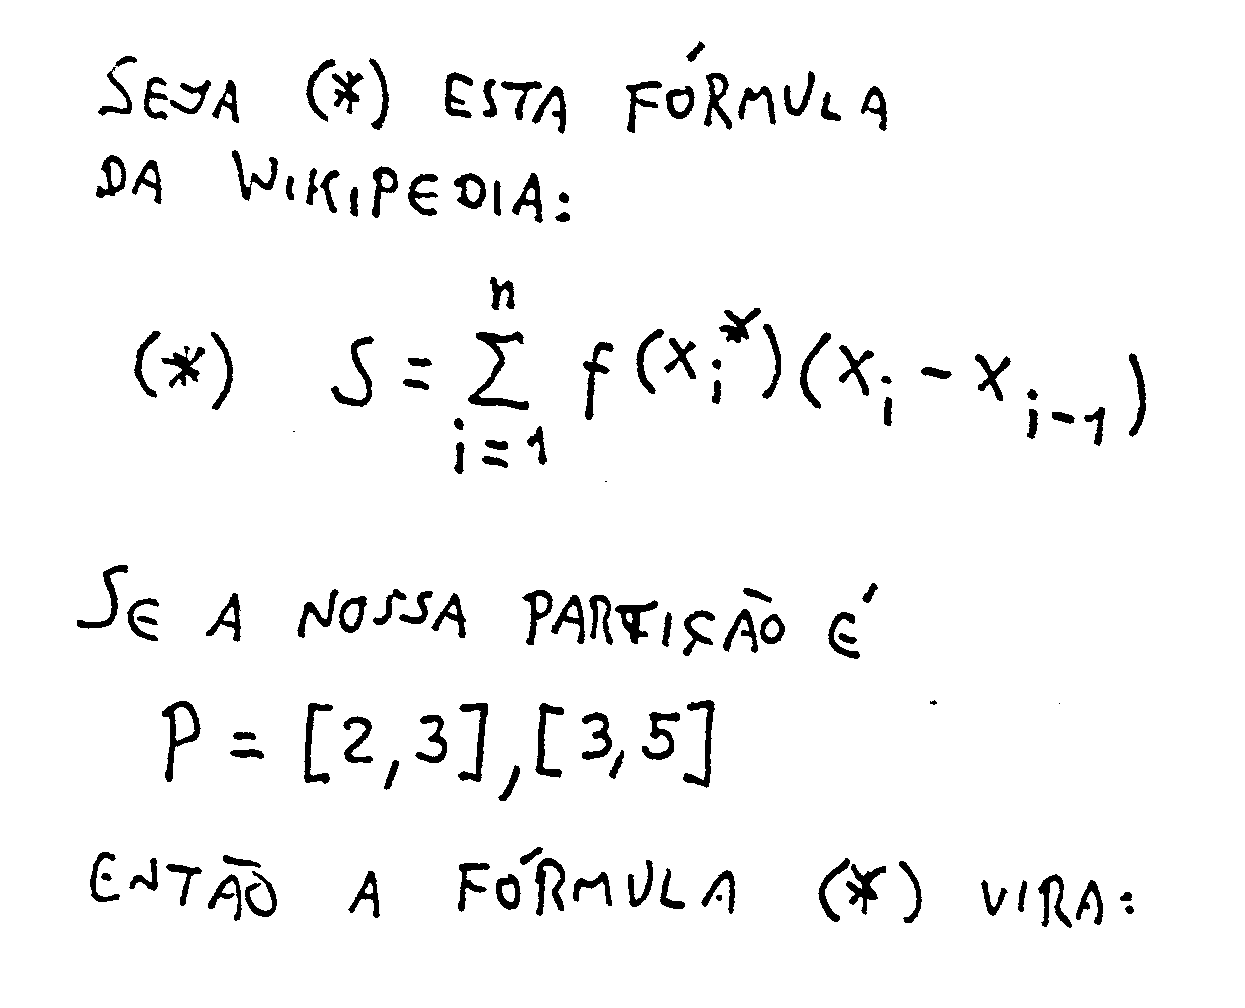
\includegraphics[height=4cm]{2021-2-C2/20211124_wp_1.pdf} \\
(Complete!) \\
\end{tabular}
%
%\qquad
%
\begin{tabular}{c}
% (find-latexscan-links "C2" "20211124_wp_2")
% (find-xpdf-page "~/LATEX/2021-2-C2/20211124_wp_2.pdf")
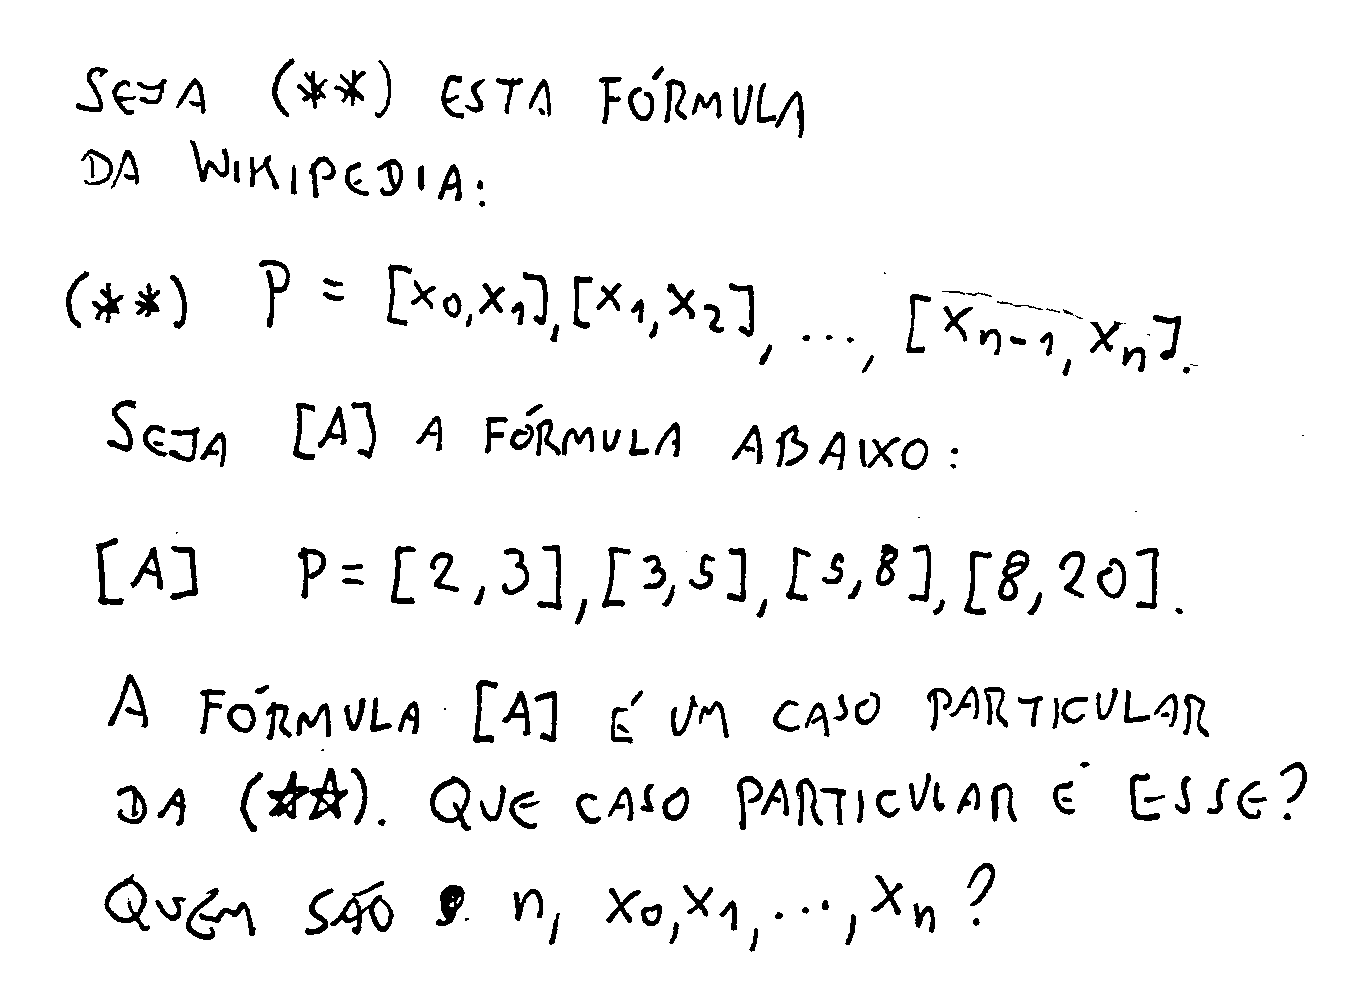
\includegraphics[height=5cm]{2021-2-C2/20211124_wp_2.pdf}
\end{tabular}

\newpage


{\bf Somatórios com `$\ldots$'s}

\scalebox{0.7}{\def\colwidth{7cm}\firstcol{

A página da Wikipedia muitas vezes usa expressões com `$\ldots$' ao
invés de somatórios (com $Σ$). A gente viu no slide 4 como a gente
consegue ``expandir um somatório'' ``pra se livrar do sinal de
`$Σ$'\,''...

\msk

A técnica pra gente expandir expressões com reticências pra se livrar
das reticências é bem mais difícil de formalizar. O scan à direita é
um exemplo.

\msk

Exercício: pegue os quatro somatórios escritos com reticências na
seção ``Método'' da Wikipedia e 1) expanda eles no caso em que $n=3$,
2) converta eles pra notação com `$Σ$'.

}\hspace*{-2cm}\def\colwidth{12cm}\anothercol{

$$\myvcenter{
% (find-latexscan-links "C2" "20211125_wp_3")
% (find-xpdf-page "~/LATEX/2021-2-C2/20211125_wp_3.pdf")
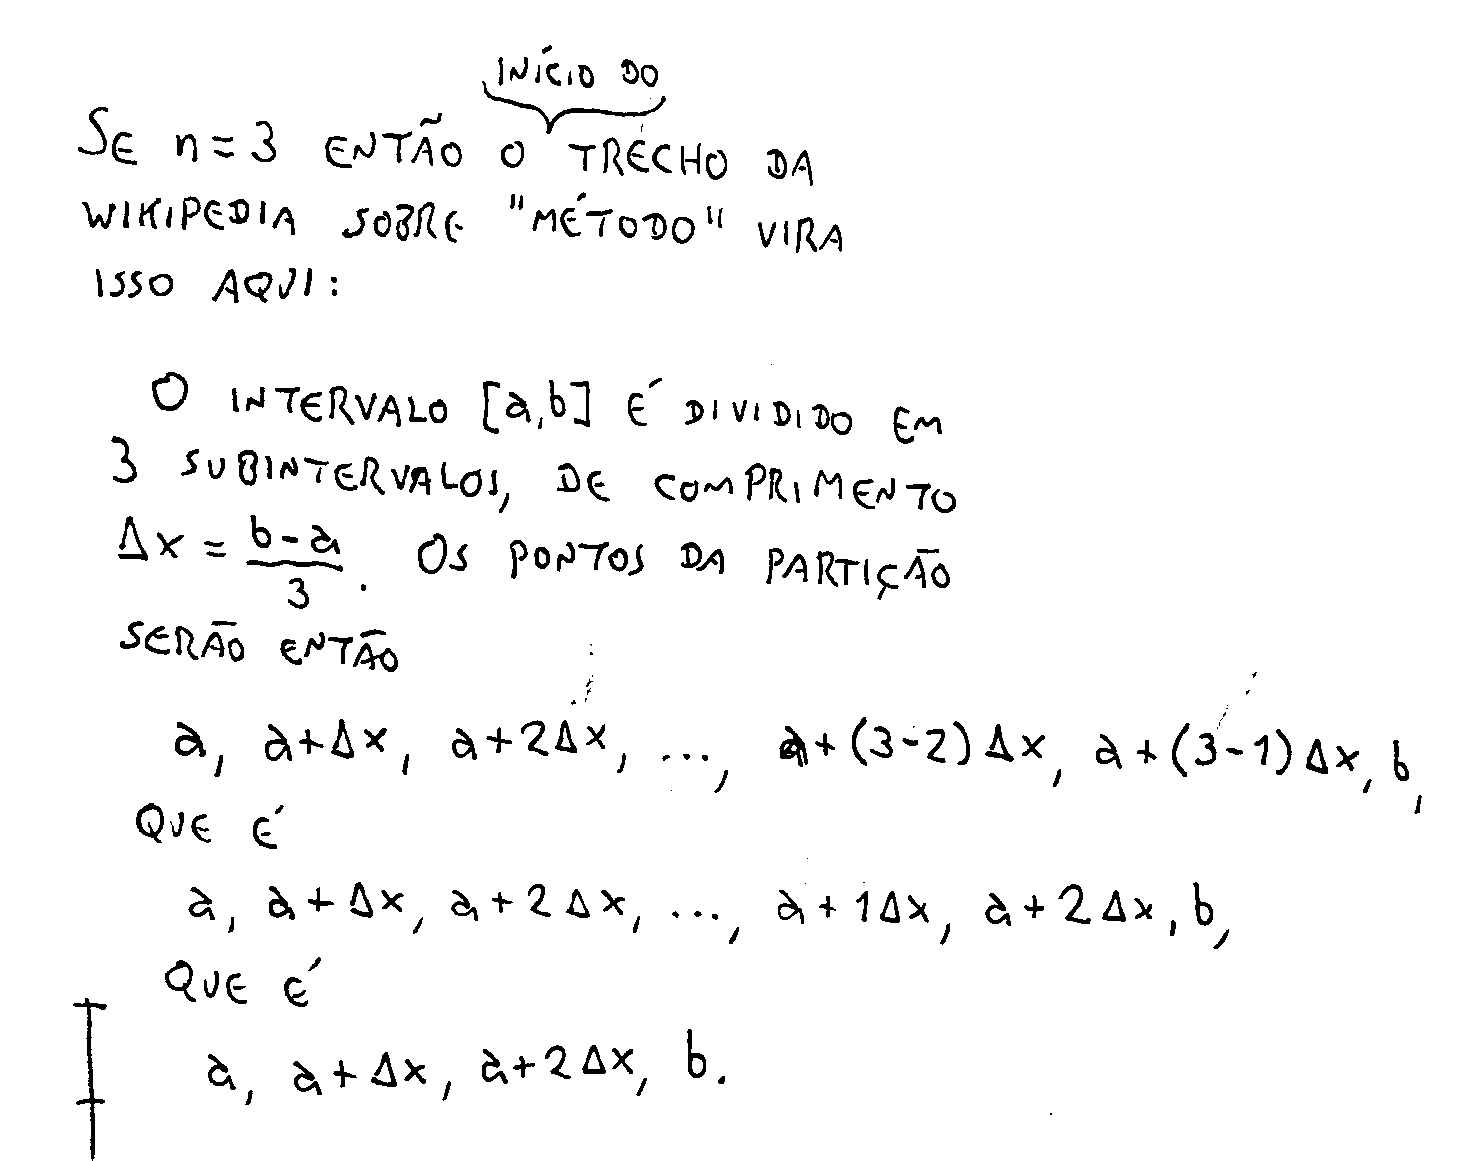
\includegraphics[height=7cm]{2021-2-C2/20211125_wp_3.pdf}
}
$$

}}


\newpage

{\bf O mini-teste}

Mostre como traduzir a notação da página sobre Somas de

Riemann da Wikipedia pra notação que eu usei nos meus PDFs.

Faça o que você puder e escreva o melhor que você puder.

Nós discutimos o que isso queria dizer nas aulas. $\smile$

\bsk



Os logs PDFizados dos canais do Telegram das turmas vão

ficar disponíveis nestes endereços aqui até sábado de noite:

\ssk

\u{http://angg.twu.net/tmp/C2-C1-RCN-PURO-2021.2.pdf}

\u{http://angg.twu.net/tmp/C2-E1-RCN-PURO-2021.2.pdf}

\ssk

As aulas da semana do mini-teste estão nas páginas 67--89

no log da turma C1 e nas páginas 67-90 no log da turma E1.







%\printbibliography

\GenericWarning{Success:}{Success!!!}  % Used by `M-x cv'

\end{document}


%  _                    
% | |    ___   __ _ ___ 
% | |   / _ \ / _` / __|
% | |__| (_) | (_| \__ \
% |_____\___/ \__, |___/
%             |___/     
%
% «upload-logs»  (to ".upload-logs")
% (c2m212mt2a         "upload-logs")
% (find-telegram-save-log-links "2021" "2" "C2" "C1")
% (find-telegram-save-log-links "2021" "2" "C2" "E1")
% http://angg.twu.net/tmp/C2-C1-RCN-PURO-2021.2.pdf
% http://angg.twu.net/tmp/C2-E1-RCN-PURO-2021.2.pdf

 (eepitch-shell)
 (eepitch-kill)
 (eepitch-shell)
Scp-np ~/2021.2-C2/C2-C1-RCN-PURO-2021.2.pdf   $TWUP/tmp/
Scp-np ~/2021.2-C2/C2-E1-RCN-PURO-2021.2.pdf   $TWUP/tmp/



% <aviso-telegram>

Gente, um aviso:

o segundo mini-teste vai ser na semana que vem e vai ser sobre
traduzir entre a notação de somas de Riemann da Wikipedia e a notação
que nós estamos usando nos PDFs, _e explicar a tradução de um jeito
que todo mundo entenda_.

Esse segundo mini-teste vai valer no máximo 0.5 pontos pra quem
participar bastante das aulas da semana que vem e no máximo 0.2 pra
quem não participar nada. Eu agora já sei como colorir as falas de
cada pessoa no log do Telegram, e aí com isso fica bem fácil reler
tudo que cada pessoa disse.



%  _                
% | |   _   _  __ _ 
% | |  | | | |/ _` |
% | |__| |_| | (_| |
% |_____\__,_|\__,_|
%                   
% «lua»  (to ".lua")
% (find-LATEX "2021-2-C2-MT2.lua")


%  ____  _             _         
% |  _ \(_)_   ___   _(_)_______ 
% | | | | \ \ / / | | | |_  / _ \
% | |_| | |\ V /| |_| | |/ /  __/
% |____// | \_/  \__,_|_/___\___|
%     |__/                       
%
% «djvuize»  (to ".djvuize")
% (find-LATEXgrep "grep --color -nH --null -e djvuize 2020-1*.tex")

 (eepitch-shell)
 (eepitch-kill)
 (eepitch-shell)
# (find-fline "~/2021.2-C2/")
# (find-fline "~/LATEX/2021-2-C2/")
# (find-fline "~/bin/djvuize")

cd /tmp/
for i in *.jpg; do echo f $(basename $i .jpg); done

f () { rm -v $1.pdf;  textcleaner -f 50 -o  5 $1.jpg $1.png; djvuize $1.pdf; xpdf $1.pdf }
f () { rm -v $1.pdf;  textcleaner -f 50 -o 10 $1.jpg $1.png; djvuize $1.pdf; xpdf $1.pdf }
f () { rm -v $1.pdf;  textcleaner -f 50 -o 20 $1.jpg $1.png; djvuize $1.pdf; xpdf $1.pdf }

f () { rm -fv $1.png $1.pdf; djvuize $1.pdf }
f () { rm -fv $1.png $1.pdf; djvuize WHITEBOARDOPTS="-m 1.0 -f 15" $1.pdf; xpdf $1.pdf }
f () { rm -fv $1.png $1.pdf; djvuize WHITEBOARDOPTS="-m 1.0 -f 30" $1.pdf; xpdf $1.pdf }
f () { rm -fv $1.png $1.pdf; djvuize WHITEBOARDOPTS="-m 1.0 -f 45" $1.pdf; xpdf $1.pdf }
f () { rm -fv $1.png $1.pdf; djvuize WHITEBOARDOPTS="-m 0.5" $1.pdf; xpdf $1.pdf }
f () { rm -fv $1.png $1.pdf; djvuize WHITEBOARDOPTS="-m 0.25" $1.pdf; xpdf $1.pdf }
f () { cp -fv $1.png $1.pdf       ~/2021.2-C2/
       cp -fv        $1.pdf ~/LATEX/2021-2-C2/
       cat <<%%%
% (find-latexscan-links "C2" "$1")
%%%
}

f 20211124_wp_1
f 20211124_wp_2
f 20211125_wp_3


%  __  __       _        
% |  \/  | __ _| | _____ 
% | |\/| |/ _` | |/ / _ \
% | |  | | (_| |   <  __/
% |_|  |_|\__,_|_|\_\___|
%                        
% <make>

 (eepitch-shell)
 (eepitch-kill)
 (eepitch-shell)
# (find-LATEXfile "2019planar-has-1.mk")
make -f 2019.mk STEM=2021-2-C2-MT2 veryclean
make -f 2019.mk STEM=2021-2-C2-MT2 pdf

% Local Variables:
% coding: utf-8-unix
% ee-tla: "c2mt2"
% ee-tla: "c2m212mt2"
% End:
